\documentclass[10pt]{article}

% ============================================================
% PACKAGES
% ============================================================

\usepackage[a4paper,margin=0.65in]{geometry}
\usepackage{amsmath,amssymb}
\usepackage{graphicx}
\usepackage{booktabs}
\usepackage{array}
\usepackage{float}
\usepackage{hyperref}
\usepackage{enumitem}
\usepackage{xcolor}
\usepackage{tikz}
\usepackage{multirow}
\usepackage{caption}
\usepackage{subcaption}

\usetikzlibrary{
positioning,
arrows.meta,
shapes.geometric,
fit,
calc
}

% ============================================================
% FORMATTING
% ============================================================

\setlist{nosep,leftmargin=*}
\renewcommand{\arraystretch}{1.2}
\setlength{\parindent}{0pt}
\setlength{\parskip}{2pt}

\hypersetup{
    colorlinks=true,
    linkcolor=blue,
    urlcolor=blue,
    citecolor=blue
}

% ============================================================
% TIKZ STYLES
% ============================================================

\tikzset{
block/.style={
draw,
rounded corners,
minimum width=1.55cm,
minimum height=0.60cm,
align=center,
fill=blue!10,
font=\scriptsize
},
attn/.style={
draw,
rounded corners,
minimum width=1.55cm,
minimum height=0.60cm,
align=center,
fill=green!12,
font=\scriptsize
},
arrow/.style={
-{Latex[length=2mm]},
thin
}
}

% ============================================================
% DOCUMENT
% ============================================================

\begin{document}

% ============================================================
% TITLE
% ============================================================

\begin{center}

{\large\textbf{Shiv Nadar University Chennai}}\\[2mm]

{\normalsize\textbf{CS3807 -- Deep Learning Laboratory}}\\[2mm]

{\large\textbf{Experiments 8, 9}}\\[1mm]

{\normalsize
\textbf{
Effect of Attention Type and Attention Position\\
in a Pretrained ResNet50
}}

\end{center}

\vspace{3mm}

% ============================================================
% COURSE DETAILS
% ============================================================

\begin{center}
\begin{tabular}{|p{3.5cm}|p{8.7cm}|p{2.1cm}|}
\hline
\textbf{Degree \& Branch}
&
B.Tech Artificial Intelligence \& Data Science
&
Semester V
\\
\hline

\textbf{Subject Code \& Name}
&
CS3807 -- Deep Learning Laboratory
&
AY: 2026--27
\\
\hline
\end{tabular}
\end{center}

% ============================================================
\section*{1. Objective}
% ============================================================

The objective of this experiment is to understand how different attention
mechanisms modify a pretrained convolutional neural network and how the
\textbf{position at which attention is inserted} influences image
classification performance.

A single pretrained architecture,

\[
\boxed{\text{ResNet50 pretrained on ImageNet}}
\]

is used throughout the experiment.

Students will investigate:

\begin{itemize}

\item channel attention;

\item spatial attention;

\item sequential channel--spatial attention;

\item lightweight self-attention;

\item different positions for inserting attention within ResNet50;

\item single-stage and multi-stage attention;

\item attention ordering;

\item additional established attention mechanisms; and

\item qualitative interpretation using internal attention maps and Grad-CAM.

\end{itemize}

The experiment emphasizes that the effectiveness of attention depends not
only on the attention mechanism itself, but also on the characteristics of
the feature representation on which it operates.

% ============================================================
\section*{2. Learning Outcomes}
% ============================================================

After completing this experiment, students will be able to:

\begin{enumerate}

\item explain the stage-wise architecture of a pretrained ResNet50;

\item distinguish early, intermediate, and late convolutional features;

\item explain the motivation behind attention mechanisms;

\item implement channel attention;

\item implement spatial attention;

\item implement sequential channel--spatial attention;

\item implement a lightweight self-attention mechanism;

\item insert an attention module at different stages of a pretrained network;

\item analyze the influence of attention position;

\item compare different attention mechanisms under a controlled experimental
protocol;

\item analyze classification accuracy and class-wise performance;

\item visualize internal attention maps;

\item generate Grad-CAM explanations;

\item distinguish an internal attention map from a post-hoc explanation map;

\item analyze accuracy--complexity trade-offs; and

\item perform controlled ablation studies.

\end{enumerate}

% ============================================================
\section*{3. Dataset}
% ============================================================

\textbf{Recommended Dataset: TensorFlow Flowers (\texttt{tf\_flowers})}

The TensorFlow Flowers dataset contains natural RGB flower images belonging
to five classes:

\begin{center}
\texttt{daisy},
\quad
\texttt{dandelion},
\quad
\texttt{roses},
\quad
\texttt{sunflowers},
\quad
\texttt{tulips}.
\end{center}

The images contain variations in:

\begin{itemize}

\item scale;

\item viewpoint;

\item illumination;

\item background clutter;

\item flower size;

\item color;

\item texture; and

\item object location.

\end{itemize}

These variations make the dataset suitable for studying the behavior of
attention mechanisms.

% ============================================================
\subsection*{3.1 Image Preprocessing}
% ============================================================

Resize every input image to

\[
224\times224\times3.
\]

The image should be preprocessed using the preprocessing procedure expected
by the ImageNet-pretrained ResNet50.

Suitable data augmentation may include:

\begin{itemize}

\item random horizontal flipping;

\item small rotations;

\item random zoom;

\item random translation; and

\item mild contrast variation.

\end{itemize}

The same augmentation strategy must be maintained for all model comparisons.

% ============================================================
\subsection*{3.2 Dataset Split}
% ============================================================

Use the same training, validation, and testing split for every experiment:

\[
\boxed{
70\% : 15\% : 15\%
}
\]

for

\[
\text{Training : Validation : Testing}.
\]

The exact same samples should be retained in each subset for all ablation
experiments.

This is necessary to ensure that differences in performance are caused by
changes in the model rather than changes in the dataset split.

% ============================================================
\section*{4. Pretrained Architecture: ResNet50}
% ============================================================

ResNet50 pretrained using ImageNet is used as the
\textbf{only backbone architecture} in this experiment.

For an input image

\[
I\in\mathbb{R}^{224\times224\times3},
\]

the major ResNet50 stages produce approximately the following feature
dimensions:

\begin{center}

\begin{tabular}{|l|c|c|}
\hline
\textbf{ResNet50 Stage}
&
\textbf{Spatial Resolution}
&
\textbf{Channels}
\\
\hline

Stem + MaxPool
&
$56\times56$
&
64
\\
\hline

conv2\_x
&
$56\times56$
&
256
\\
\hline

conv3\_x
&
$28\times28$
&
512
\\
\hline

conv4\_x
&
$14\times14$
&
1024
\\
\hline

conv5\_x
&
$7\times7$
&
2048
\\
\hline

\end{tabular}

\end{center}

As the network becomes deeper:

\[
\boxed{
\text{Spatial Resolution}\downarrow
}
\]

while

\[
\boxed{
\text{Feature Channels}\uparrow
}
\]

and the representation generally progresses from low-level visual
information toward higher-level semantic information.

% ============================================================
\section*{5. Understanding ResNet50 Feature Hierarchy}
% ============================================================

The approximate interpretation of different stages is:

\begin{itemize}

\item \textbf{Early features:}
edges, colors, orientations, boundaries, and simple textures.

\item \textbf{Intermediate features:}
local patterns, repeated structures, flower parts, petal arrangements, and
shape information.

\item \textbf{Late features:}
high-level object structures and class-discriminative semantic information.

\end{itemize}

Therefore, the same attention mechanism may produce different behavior when
inserted at different locations.

% ============================================================
\section*{6. Why Attention Position Matters}
% ============================================================

Attention is not independent of the features on which it operates.

Suppose an attention module receives

\[
F\in\mathbb{R}^{H\times W\times C}.
\]

The values of

\[
H,\qquad W,\qquad C
\]

and the semantic meaning of the feature tensor change significantly with
network depth.

Therefore:

\begin{itemize}

\item \textbf{early-stage attention} operates on high-resolution,
low-level visual information;

\item \textbf{middle-stage attention} operates on intermediate features
containing both spatial and semantic information; and

\item \textbf{late-stage attention} operates on low-resolution,
high-level semantic representations.

\end{itemize}

Thus, students should investigate both:

\[
\boxed{\text{Which attention mechanism should be used?}}
\]

and

\[
\boxed{\text{Where should the attention mechanism be inserted?}}
\]

% ============================================================
\section*{7. Candidate Attention Positions}
% ============================================================

Define four candidate attention positions in ResNet50.

\[
P_1:
\text{ after conv2\_x},
\]

\[
P_2:
\text{ after conv3\_x},
\]

\[
P_3:
\text{ after conv4\_x},
\]

\[
P_4:
\text{ after conv5\_x}.
\]

The corresponding feature dimensions are:

\begin{center}

\begin{tabular}{|c|c|c|c|}
\hline

\textbf{Position}
&
\textbf{Location}
&
\textbf{Resolution}
&
\textbf{Channels}
\\
\hline

$P_1$
&
After conv2\_x
&
$56\times56$
&
256
\\
\hline

$P_2$
&
After conv3\_x
&
$28\times28$
&
512
\\
\hline

$P_3$
&
After conv4\_x
&
$14\times14$
&
1024
\\
\hline

$P_4$
&
After conv5\_x
&
$7\times7$
&
2048
\\
\hline

\end{tabular}

\end{center}

For the principal laboratory exercise, students should concentrate on

\[
\boxed{
P_2,\quad P_3,\quad P_4
}
\]

because $P_1$ contains comparatively high-resolution features and may
substantially increase the computational cost of some attention mechanisms.

% ============================================================
\section*{8. Baseline Model}
% ============================================================

The baseline is the pretrained ResNet50 without any additional attention
mechanism.

\begin{center}

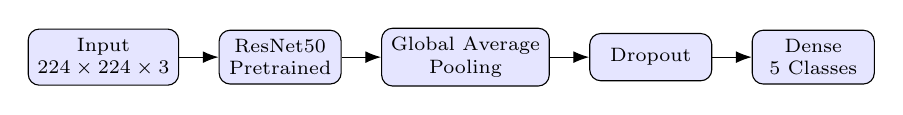
\begin{tikzpicture}[node distance=5mm]

\node[block] (a)
{Input\\$224\times224\times3$};

\node[block,right=of a] (b)
{ResNet50\\Pretrained};

\node[block,right=of b] (c)
{Global Average\\Pooling};

\node[block,right=of c] (d)
{Dropout};

\node[block,right=of d] (e)
{Dense\\5 Classes};

\foreach \x/\y in {a/b,b/c,c/d,d/e}
\draw[arrow] (\x)--(\y);

\end{tikzpicture}

\end{center}

The baseline establishes the reference performance against which the
attention-based models are compared.

% ============================================================
\section*{9. Channel Attention}
% ============================================================

Consider a feature tensor

\[
F\in\mathbb{R}^{H\times W\times C}.
\]

Channel attention determines the relative importance of different feature
channels.

Global average pooling is first used to generate a channel descriptor:

\[
z_c
=
\frac{1}{HW}
\sum_{i=1}^{H}
\sum_{j=1}^{W}
F(i,j,c).
\]

Thus,

\[
z\in\mathbb{R}^{C}.
\]

The channel descriptor is transformed using two learnable transformations:

\[
M_c(F)
=
\sigma
\left(
W_2
\delta
\left(
W_1z
\right)
\right),
\]

where:

\begin{itemize}

\item $\delta(\cdot)$ denotes a nonlinear activation such as ReLU;

\item $\sigma(\cdot)$ denotes the sigmoid activation;

\item $W_1$ reduces the channel representation; and

\item $W_2$ restores the channel dimension.

\end{itemize}

The refined feature tensor is:

\[
F_c
=
F\odot M_c(F).
\]

Channel attention attempts to answer:

\[
\boxed{\text{Which feature channels are important?}}
\]

A reduction ratio of

\[
r=16
\]

may be used as the default setting throughout the laboratory experiment.

The reduction ratio need not be treated as a separate mandatory ablation.

% ============================================================
\section*{10. Spatial Attention}
% ============================================================

Spatial attention determines the spatial regions that should receive greater
importance.

For the input feature tensor

\[
F\in\mathbb{R}^{H\times W\times C},
\]

compute average pooling across channels:

\[
F_{\mathrm{avg}}
=
\operatorname{Mean}_{c}(F),
\]

and maximum pooling across channels:

\[
F_{\mathrm{max}}
=
\operatorname{Max}_{c}(F).
\]

Both tensors have dimensions

\[
H\times W\times1.
\]

Concatenate them:

\[
F_s
=
[
F_{\mathrm{avg}}
\Vert
F_{\mathrm{max}}
].
\]

The spatial attention map is then computed as

\[
M_s(F)
=
\sigma
\left(
\operatorname{Conv}_{7\times7}(F_s)
\right).
\]

Therefore,

\[
M_s(F)
\in
\mathbb{R}^{H\times W\times1}.
\]

The spatially refined feature is

\[
F_s'
=
F\odot M_s(F).
\]

Spatial attention answers:

\[
\boxed{\text{Which spatial locations are important?}}
\]

% ============================================================
\section*{11. Sequential Channel--Spatial Attention}
% ============================================================

Channel and spatial attention can be sequentially applied.

First,

\[
F_c
=
M_c(F)\odot F.
\]

Then,

\[
F_{cs}
=
M_s(F_c)\odot F_c.
\]

The overall structure becomes:

\[
\boxed{
F
\rightarrow
\text{Channel Attention}
\rightarrow
\text{Spatial Attention}
\rightarrow
F_{cs}
}
\]

This arrangement first determines

\[
\text{``what is important''}
\]

and then determines

\[
\text{``where it is important.''}
\]

A simplified diagram is shown below.

\begin{center}

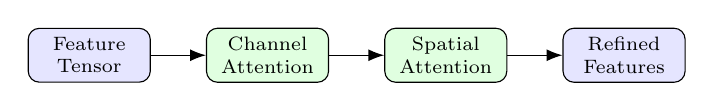
\begin{tikzpicture}[node distance=7mm]

\node[block] (a)
{Feature\\Tensor};

\node[attn,right=of a] (b)
{Channel\\Attention};

\node[attn,right=of b] (c)
{Spatial\\Attention};

\node[block,right=of c] (d)
{Refined\\Features};

\draw[arrow] (a)--(b);
\draw[arrow] (b)--(c);
\draw[arrow] (c)--(d);

\end{tikzpicture}

\end{center}

% ============================================================
\section*{12. Self-Attention}
% ============================================================

Self-attention allows spatial locations to interact directly with other
spatial locations.

For

\[
F\in\mathbb{R}^{H\times W\times C},
\]

flatten the spatial dimensions:

\[
X\in\mathbb{R}^{N\times C},
\]

where

\[
N=HW.
\]

Generate the query, key, and value matrices:

\[
Q=XW_Q,
\]

\[
K=XW_K,
\]

and

\[
V=XW_V.
\]

The attention matrix is

\[
A
=
\operatorname{softmax}
\left(
\frac{QK^T}{\sqrt{d}}
\right),
\]

where $d$ is the dimension of the query/key representation.

The attended output is

\[
Y=AV.
\]

After reshaping the output back to the original spatial structure, a residual
formulation may be used:

\[
F_{\mathrm{SA}}
=
F
+
\gamma
\operatorname{reshape}(Y),
\]

where $\gamma$ is a learnable scaling parameter.

Self-attention attempts to answer:

\[
\boxed{
\text{Which spatial features are related to other spatial features?}
}
\]

Since the attention matrix has dimension approximately

\[
N\times N,
\]

its computational requirements increase rapidly as

\[
N=HW
\]

increases.

Therefore, self-attention should preferably be introduced at

\[
P_3
\]

or

\[
P_4.
\]

% ============================================================
\section*{13. Inserting Attention into ResNet50}
% ============================================================

For any selected stage $P_k$, the network structure can be written as

\[
\text{Previous ResNet Stage}
\rightarrow
\text{Attention}
\rightarrow
\text{Next ResNet Stage}.
\]

For example, attention inserted after conv4\_x gives:

\[
\boxed{
\text{conv4\_x}
\rightarrow
\text{Attention}
\rightarrow
\text{conv5\_x}
}
\]

For channel--spatial attention:

\[
\boxed{
\text{conv4\_x}
\rightarrow
\text{Channel Attention}
\rightarrow
\text{Spatial Attention}
\rightarrow
\text{conv5\_x}
}
\]

The student must record the feature dimensions immediately before and after
the attention block.

Attention should not unintentionally modify the spatial or channel
dimensions unless the selected mechanism explicitly requires such a
transformation.

% ============================================================
\section*{14. Main Experiment 1: Attention-Type Ablation}
% ============================================================

The first experiment studies the effect of different types of attention.

Fix the attention position at

\[
\boxed{
P_3=\text{after conv4\_x}
}
\]

for all models.

Compare the following:

\begin{center}

\begin{tabular}{|l|c|c|c|}
\hline

\textbf{Model}
&
\textbf{Channel}
&
\textbf{Spatial}
&
\textbf{Self-Attention}
\\
\hline

A0: Baseline ResNet50
&
--
&
--
&
--
\\
\hline

A1: Channel Attention
&
$\checkmark$
&
--
&
--
\\
\hline

A2: Spatial Attention
&
--
&
$\checkmark$
&
--
\\
\hline

A3: Channel+Spatial
&
$\checkmark$
&
$\checkmark$
&
--
\\
\hline

A4: Self-Attention
&
--
&
--
&
$\checkmark$
\\
\hline

A5: Combined Attention
&
$\checkmark$
&
$\checkmark$
&
$\checkmark$
\\
\hline

\end{tabular}

\end{center}

This experiment investigates:

\[
\boxed{
\text{How does attention type affect model performance?}
}
\]

Students must keep the following identical:

\begin{itemize}

\item dataset split;

\item preprocessing;

\item augmentation;

\item optimizer;

\item learning rate schedule;

\item epochs;

\item batch size;

\item backbone;

\item classifier;

\item attention position; and

\item evaluation procedure.

\end{itemize}

\begin{figure}[H]
\centering
\includegraphics[width=0.85\linewidth]
{attention_type_comparison.eps}
\caption{Performance comparison of baseline ResNet50 and
attention-based models at P3.}
\label{fig:attention_type_comparison}
\end{figure}

\textbf{Inference:}

Spatial attention yielded the best macro F1 score of 0.9204. Spatial attention and self-attention both gave 92.01\% accuracy. SE (channel) attention increased the accuracy above the baseline from 90.93\% to 91.65\%. CBAM at P3 resulted in an accuracy of 89.84\%, less than the baseline. Hence, attention does not ensure better results. It all depends on the method used and where it is applied.


\begin{figure}[H]
\centering
\includegraphics[width=0.78\linewidth]{baseline_accuracy.eps}
\caption{Training and validation accuracy of baseline ResNet50.}
\end{figure}

\textbf{Inference:}
The chart represents the dynamics of baseline training and validation accuracy. Comparison between the two curves allows determining whether improvements in training are also observed on the validation set. A consistent difference between the two curves may be regarded as a sign of the generalization gap. The behavior at the last epoch cannot be established from the source text.


\begin{figure}[H]
\centering
\includegraphics[width=0.78\linewidth]{baseline_loss.eps}
\caption{Training and validation loss of baseline ResNet50.}
\end{figure}

\textbf{Inference:}
The plot shows categorical cross-entropy during baseline training. Loss decrease means that error in predictions on the particular dataset is decreasing. An increasing difference between training and validation losses may indicate overfitting. Exact loss values and occurrence of overfitting can only be concluded from the plot, not from the text.

\begin{figure}[H]
\centering
\includegraphics[width=0.88\linewidth]
{training_accuracy_comparison.eps}
\caption{Training and validation accuracy across attention models.}
\end{figure}

\textbf{Inference:}
In this figure, learning behaviors of the baseline and attention models are compared. Validation accuracy plays a vital role in making generalization comparisons. High training accuracy does not necessarily mean a model will perform well on unseen images. Exact convergence time and the best-performing curve cannot be known without looking at the figure.


\begin{figure}[H]
\centering
\includegraphics[width=0.95\linewidth]
{all_models_confusion_matrices.eps}
\caption{Confusion matrices for the evaluated attention models.}
\label{fig:attention_confusion_matrices}
\end{figure}

\textbf{Inference:}

The confusion matrices offer class-specific information that is not conveyed using only accuracy. The diagonal elements correspond to correctly classified instances, while off-diagonal elements reflect incorrect classifications. Comparison of the confusion matrices for the baseline and attention mechanisms helps understand whether classification errors for each class vary across models. Spatial attention yielded accuracy of 0.9201, whereas the baseline had 0.9093. Finding which flower classes gained the most from attention can be done only by observing the matrices.

\begin{figure}[H]
\centering
\includegraphics[width=0.85\linewidth]
{se_p3_channel_weights.eps}
\caption{Channel-attention weights for SE at P3.}
\end{figure}

\textbf{Inference:}

SE gives different weights to the feature channels instead of treating all channels the same. Higher weights mean higher emphasis on these channels through the attention mechanism. Weights denote the relative importance of channels in the learned representation. They do not indicate which human-understandable objects or image parts the channels represent.

\begin{figure}[H]
\centering
\includegraphics[width=0.90\linewidth]
{gradcam_baseline_vs_cbam_p3.eps}
\caption{Grad-CAM comparison between baseline ResNet50 and CBAM at P3.}
\label{fig:gradcam_exp1}
\end{figure}

\textbf{Inference:}

Grad-CAM indicates the image parts which help in the prediction of the class in question. Comparing the baseline and CBAM heatmaps is needed to figure out whether the models focus on the same or different image regions. The heatmaps must be studied to check whether activation happens on the flower, petals, leaves, or background. Concentration of the heatmap does not guarantee better classification or explanation.

The second experiment investigates the influence of the position
of attention on image classification performance.

The attention type is fixed as:

\[
\boxed{
\text{Channel Attention}
\rightarrow
\text{Spatial Attention}
}
\]

The same Channel and Spatial Attention module (CBAM) is inserted
at different stages of the ResNet50 backbone. This experiment
studies whether attention is more beneficial when applied to
high-resolution low-level features, intermediate representations,
or low-resolution semantic features.

\begin{center}
\begin{tabular}{|l|l|c|c|}
\hline
\textbf{Experiment}
&
\textbf{Attention Position}
&
\textbf{Resolution}
&
\textbf{Channels}
\\
\hline
B1 & After conv2\_x & $56\times56$ & 256 \\
\hline
B2 & After conv3\_x & $28\times28$ & 512 \\
\hline
B3 & After conv4\_x & $14\times14$ & 1024 \\
\hline
B4 & After conv5\_x & $7\times7$ & 2048 \\
\hline
\end{tabular}
\end{center}

The principal objective is to determine how the location of the
attention module influences classification accuracy, macro
precision, macro recall, macro F1-score, model parameters, and
inference time.

\[
\boxed{
\text{How does the location of attention influence performance?}
}
\]

% ------------------------------------------------------------
% Attention Position Performance Comparison
% ------------------------------------------------------------

\begin{figure}[H]
\centering
\includegraphics[width=0.85\linewidth]
{cbam_position_comparison.eps}
\caption{Performance comparison of CBAM attention applied at
different network positions.}
\label{fig:cbam_position_comparison}
\end{figure}

\textbf{Inference:}

CBAM at P4 gives the highest accuracy of 92.01\% and macro F1-score of 0.9210. CBAM at P2 has accuracy of 90.20\% and macro F1 of 0.9031. CBAM at P3 gives accuracy of 89.84\% and macro F1 of 0.8986. P4 outperformed P2 and P3 in this experiment. In this particular experiment, using CBAM in a later stage (P4), with lower-resolution features, yielded better performance than P2 or P3. This concerns these particular CBAM settings and does not guarantee that P4 will always be best for every attention mechanism.

\begin{figure}[H]
\centering
\includegraphics[width=0.85\linewidth]
{spatial_attention_p2_p3_p4.eps}
\caption{Effect of Spatial Attention Position on Classification
Performance.}
\label{fig:spatial_attention_position}
\end{figure}

\textbf{Inference:}

The visualization shows the difference in spatial attention for various ResNet50 stages. These maps can be analyzed to find changes in emphasized image parts depending on the network stage. Early stages preserve higher spatial resolution, while deeper stages work with features with lower spatial resolution. Claims related to petals, flower centers, or background emphasis should be backed up by analysis of the maps shown.


\begin{table}[H]
\centering
\caption{Performance Comparison for Different CBAM Attention Positions}
\label{tab:cbam_position_results}
\resizebox{\textwidth}{!}{
\begin{tabular}{|c|c|c|c|c|r|c|}
\hline
\textbf{Position} &
\textbf{Accuracy} &
\textbf{Precision} &
\textbf{Recall} &
\textbf{Macro F1} &
\textbf{Parameters} &
\textbf{Inference Time} \\
\hline
$P_2$ & 0.9020 & 0.9075 & 0.9021 & 0.9031 & 23,631,367 & 29.5933 ms \\
\hline
$P_3$ & 0.8984 & 0.9050 & 0.8976 & 0.8986 & 23,730,215 & 29.5569 ms \\
\hline
$P_4$ & 0.9201 & 0.9215 & 0.9211 & 0.9210 & 24,124,519 & 29.7718 ms \\
\hline
\end{tabular}
}
\end{table}

\textbf{Inference:}

P4 was the best-performing model in this position experiment in terms of both accuracy and macro F1-score. It surpassed P2 by 1.81 percentage points in accuracy and P3 by 2.17 percentage points. P4 also had the largest number of parameters and inference time among the three models. However, P3 was faster than P2 but had the worst accuracy and macro F1-score among them. The example demonstrated a trade-off between performance and complexity.


% ============================================================
\section*{16. Main Experiment 3: Multiple Attention Positions}
% ============================================================

Attention may also be inserted at more than one ResNet50 stage.

Compare:

\[
\text{Attention only at }P_3,
\]

\[
\text{Attention only at }P_4,
\]

and

\[
\text{Attention at }P_3+P_4.
\]

As an extended experiment, students may evaluate:

\[
P_2+P_3+P_4.
\]

The purpose is to investigate whether applying attention repeatedly provides
sufficient performance improvement to justify the additional:

\begin{itemize}

\item parameters;

\item computation;

\item memory;

\item training time; and

\item inference time.

\end{itemize}

Students should experimentally answer:

\[
\boxed{
\text{Is attention at more locations necessarily more effective?}
}
\]

\begin{table}[H]
\centering
\caption{Performance Comparison of Single-Stage and Multi-Stage CBAM}
\label{tab:multi_stage_attention}
\resizebox{\textwidth}{!}{
\begin{tabular}{|c|c|c|c|c|}
\hline
\textbf{Attention Configuration} &
\textbf{Accuracy} &
\textbf{Macro Precision} &
\textbf{Macro Recall} &
\textbf{Macro F1-score} \\
\hline
CBAM ($P_3$) & 0.8984 & 0.9050 & 0.8976 & 0.8986 \\
\hline
CBAM ($P_4$) & 0.9201 & 0.9215 & 0.9211 & 0.9210 \\
\hline
CBAM ($P_3+P_4$) & 0.9201 & 0.9230 & 0.9202 & 0.9207 \\
\hline
\end{tabular}
}
\end{table}

\textbf{Inference:}

Both CBAM at P4 and CBAM at P3 + P4 reached accuracy of 92.01\%. P4 only had a slightly better macro F1-score: 0.9210 against 0.9207. While the multi-stage configuration reached the best macro precision value of 0.9230, it could not surpass P4 only in overall accuracy or macro F1-score. The multi-stage model had 24,256,777 parameters, against 24,124,519 for P4 only. Thus, adding another attention layer provided no evident performance improvement in this experiment, even though it made the network more complex.

\begin{figure}[H]
\centering
\includegraphics[width=0.85\linewidth]
{multi_stage_attention_comparison.eps}
\caption{Comparison of Test Accuracy and Macro F1-score for
Single-Stage and Multi-Stage CBAM.}
\label{fig:multi_stage_attention_comparison}
\end{figure}

\textbf{Inference:}

The chart shows accuracy and macro F1-score for different single-stage and multi-stage CBAM configurations. P4 and P3 + P4 have identical accuracy, while P4 has the slightly better macro F1-score. These results do not support the assumption that adding attention at more stages will be beneficial for classification. Configuration choice should be based on precision, recall, F1-score, and complexity rather than accuracy alone.

% ============================================================
\section*{17. Main Experiment 4: Attention Order}
% ============================================================

The sequence in which channel and spatial attention are applied may influence
the resulting features.

Compare:

\[
\boxed{
\text{Channel}
\rightarrow
\text{Spatial}
}
\]

against

\[
\boxed{
\text{Spatial}
\rightarrow
\text{Channel}
}
\]

while maintaining the same insertion position.

For example, at $P_3$:

\[
F
\rightarrow
M_c
\rightarrow
M_s
\]

should be compared with

\[
F
\rightarrow
M_s
\rightarrow
M_c.
\]

Students should determine whether selecting informative feature channels
before selecting spatial regions produces behavior different from selecting
spatial regions first.

\begin{table}[H]
\centering
\caption{Effect of Attention Order on Classification Performance at $P_3$}
\label{tab:attention_order}
\resizebox{\textwidth}{!}{
\begin{tabular}{|l|c|c|c|c|c|}
\hline
\textbf{Attention Order} &
\textbf{Accuracy} &
\textbf{Macro Precision} &
\textbf{Macro Recall} &
\textbf{Macro F1-score} &
\textbf{Parameters} \\
\hline
Channel $\rightarrow$ Spatial
& 0.9074 & 0.9135 & 0.9058 & 0.9075 & 23,730,215 \\
\hline
Spatial $\rightarrow$ Channel
& 0.9220 & 0.9294 & 0.9198 & 0.9226 & 23,730,215 \\
\hline
\end{tabular}
}
\end{table}

\textbf{Inference:}

Spatial-first attention outperformed channel-first attention in all four classification metrics mentioned. Accuracy improved from 90.74\% to 92.20\%, which amounts to 1.46 percentage points gained. Macro F1-score improved from 0.9075 to 0.9226. Spatial-first attention also had greater macro precision and recall. The number of parameters in both cases was 23,730,215. With the parameter counts being equal, attention operation ordering was an essential factor in this comparison. At position P3, spatial attention followed by channel attention performed better.

\begin{figure}[H]
\centering
\includegraphics[width=0.85\linewidth]
{attention_order_comparison.eps}
\caption{Comparison of Channel-First and Spatial-First Attention at $P_3$.}
\label{fig:attention_order_comparison}
\end{figure}

\textbf{Inference:}

The chart provides a visualization of channel-first and spatial-first attention. The numerical results show that spatial-first attention produced higher accuracy and macro F1-score. The graph needs to be analyzed along with the table because the two cases have equal parameter counts but different classification metrics. The conclusion about spatial-first ordering is justified by this case; however, more runs are needed to confirm the advantage across different random seeds.

% ============================================================
\section*{18. Main Experiment 5: Spatial Attention Kernel Size}
% ============================================================

The receptive field used to generate the spatial attention map may influence
the result.

Evaluate:

\[
k\in\{3,5,7\}.
\]

Use the same attention position and training protocol.

\begin{center}




\begin{table}[H]
\centering
\caption{Classification Performance for Different Spatial Attention Kernel Sizes}
\label{tab:kernel_size_results}
\resizebox{\textwidth}{!}{
\begin{tabular}{|c|c|c|c|c|}
\hline
\textbf{Kernel Size}
&
\textbf{Accuracy}
&
\textbf{Macro Precision}
&
\textbf{Macro Recall}
&
\textbf{Macro F1-score}
\\
\hline
$3\times3$ & 0.9129 & 0.9199 & 0.9106 & 0.9135 \\
\hline
$5\times5$ & 0.8984 & 0.9072 & 0.8963 & 0.8988 \\
\hline
$7\times7$ & 0.9020 & 0.9105 & 0.8998 & 0.9019 \\
\hline
\end{tabular}
}
\end{table}

\textbf{Inference:}

The 3×3 kernel had the best accuracy, macro precision, macro recall, and macro F1-score among the three kernels. Its accuracy was 1.45 percentage points higher than the 5×5 kernel and 1.09 percentage points higher than the 7×7 kernel. The 5×5 kernel had the lowest results in all four metrics. Growing the kernel size did not lead to any improvements in classification accuracy. Since there are no inference-time and parameter comparisons for the three kernel sizes, we cannot say which kernel is the most computationally efficient one.


\end{center}

Students should discuss whether a larger spatial kernel provides a useful
increase in contextual information.

% ============================================================
\section*{19. Additional Task: Comparison of Different Attention Mechanisms}
% ============================================================

As an additional exploration task, students should compare the attention
mechanisms implemented in the laboratory with established attention
approaches.

Students should select at least

\[
\boxed{\text{two additional attention mechanisms}}
\]

from the following:

\begin{itemize}

\item Squeeze-and-Excitation (SE) Attention;

\item Efficient Channel Attention (ECA);

\item Convolutional Block Attention Module (CBAM);

\item Coordinate Attention; and

\item lightweight Self-Attention.

\end{itemize}

The pretrained backbone must remain:

\[
\boxed{\text{ResNet50}}
\]

for all comparisons.

To ensure a fair comparison, additional attention mechanisms should
preferably be inserted at the same position:

\[
\boxed{
P_3=\text{after conv4\_x}
}
\]

unless the student provides a technical justification for using another
location.

% ============================================================
\subsection*{19.1 Suggested Comparison}
% ============================================================

\begin{center}
\resizebox{\textwidth}{!}{%
\begin{tabular}{|l|c|c|c|c|c|c|}
\hline
\textbf{Attention Mechanism} &
\textbf{Accuracy} &
\textbf{Precision} &
\textbf{Recall} &
\textbf{Macro F1} &
\textbf{Parameters} &
\textbf{Inference Time} \\
\hline

No Attention & 0.9093 & 0.9173 & 0.9086 & 0.9107 & 23,597,957 & 27.7320 ms \\
\hline

Channel / SE & 0.9165 & 0.9200 & 0.9167 & 0.9169 & 23,730,117 & 27.6971 ms \\
\hline

Spatial Attention & 0.9201 & 0.9248 & 0.9185 & 0.9204 & 23,598,055 & 27.7923 ms \\
\hline

CBAM & 0.8984 & 0.9050 & 0.8976 & 0.8986 & 23,730,215 & 29.5569 ms \\
\hline

Self-Attention & 0.9201 & 0.9230 & 0.9195 & 0.9203 & 24,123,653 & 29.1271 ms \\
\hline

\end{tabular}%
}
\end{center}

\begin{figure}[H]
\centering
\includegraphics[width=0.9\linewidth]
{all_model_performance_comparison.eps}
\caption{Classification Performance Comparison of Attention Models.}
\label{fig:all_attention_performance}
\end{figure}

\begin{figure}[H]
\centering
\includegraphics[width=0.85\linewidth]
{parameter_comparison.eps}
\caption{Comparison of Model Parameters Across Attention Mechanisms.}
\label{fig:attention_parameters}
\end{figure}

\begin{figure}[H]
\centering
\includegraphics[width=0.85\linewidth]
{inference_time_comparison.eps}
\caption{Inference Time Comparison of Attention Models.}
\label{fig:attention_inference_time}
\end{figure}

\textbf{Inference:}

SE achieved the minimum inference time, at 27.6971 ms per image. Baseline inference time was 27.7320 ms per image; spatial attention took 27.7923 ms per image. Self-attention needed 29.1271 ms per image, and CBAM at P3 took 29.5569 ms per image. Spatial attention was more accurate than the baseline with little increase in inference time. CBAM at P3 was less accurate and slower than the baseline. These times are based on the measured setup and are not universal latency values for other systems.

CBAM at position $P_3$ achieved 89.84\% accuracy, which was
lower than the baseline in this experiment. In terms of model
complexity, spatial attention introduced very few additional
parameters compared with the baseline. Self-attention achieved
competitive classification performance but required more
parameters than the baseline and SE models.

The measured inference times ranged from approximately
27.70 to 29.56 milliseconds per image for the five compared
models. SE had the lowest measured inference time, while
CBAM at $P_3$ had the highest. These results show that a more
complex attention mechanism does not necessarily provide
better classification performance. Spatial attention provided
the strongest macro F1-score with only a small increase in
the total parameter count.

% ============================================================
\subsection*{19.2 Questions for Attention-Mechanism Comparison}
% ============================================================

Students should investigate:



\begin{enumerate}

\item \textbf{How does classification accuracy vary across attention mechanisms?}

Spatial attention and self-attention achieved the highest
accuracy of 92.01\%. SE achieved 91.65\%, while CBAM achieved
89.84\%. The baseline ResNet50 achieved 90.93\%.

\item \textbf{How does macro F1-score vary across attention mechanisms?}

Spatial attention achieved the highest macro F1-score of
0.9204, followed closely by self-attention at 0.9203.
SE achieved 0.9169, while CBAM achieved 0.8986.

\item \textbf{How many parameters are introduced by each attention module?}

The baseline contained 23,597,957 parameters. SE contained
23,730,117 parameters, spatial attention contained
23,598,055 parameters, CBAM contained 23,730,215 parameters,
and self-attention contained 24,123,653 parameters.

\item \textbf{How does each attention mechanism influence inference time?}

The measured inference times were 27.7320 ms/image for the
baseline, 27.6971 ms/image for SE, 27.7923 ms/image for
spatial attention, 29.5569 ms/image for CBAM, and
29.1271 ms/image for self-attention.

\item \textbf{Does attention improve convergence behavior?}

The recorded training curves can be used to compare convergence.
However, the final evaluation metrics alone are insufficient
to establish that every attention mechanism converges faster
than the baseline.

\item \textbf{Does attention produce more focused feature localization?}

Attention mechanisms reweight feature responses to emphasize
relevant information. The Grad-CAM comparison can provide
visual evidence of localization differences, although the
classification metrics alone do not establish improved
localization.

\item \textbf{Does an increase in attention complexity always improve classification performance?}

No. Self-attention used more parameters than spatial attention
but achieved a slightly lower macro F1-score. CBAM also had
more parameters than the baseline but achieved lower accuracy
in this experiment.

\item \textbf{Does a lightweight attention mechanism provide comparable performance with a computationally heavier mechanism?}

Yes. Spatial attention achieved 92.01\% accuracy and a macro
F1-score of 0.9204 with only 98 additional parameters compared
with the baseline. This was comparable to self-attention,
which achieved the same accuracy with a substantially larger
parameter count.

\end{enumerate}

The objective is to understand:

\[
\boxed{
\text{Performance}
+
\text{Complexity}
+
\text{Attention Behaviour}
}
\]

rather than considering only classification accuracy.




% ============================================================
\section*{20. Transfer-Learning Strategy}
% ============================================================

Use ImageNet pretrained weights.

A recommended training strategy is:

\begin{enumerate}

\item Load ResNet50 with ImageNet pretrained weights.

\item Remove the original ImageNet classification layer.

\item Insert the selected attention module.

\item Add Global Average Pooling.

\item Add Dropout.

\item Add a Dense classification layer containing five output neurons.

\item Initially freeze the pretrained ResNet50 layers.

\item Train the newly introduced attention and classification layers.

\item Unfreeze the final ResNet50 stage or selected final stages.

\item Fine-tune the network using a smaller learning rate.

\end{enumerate}

A suitable initial learning rate for the newly introduced layers is

\[
10^{-3}.
\]

During fine-tuning, a smaller learning rate such as

\[
10^{-5}
\quad\text{to}\quad
10^{-4}
\]

may be used.

The exact values selected by the student should remain identical for all
controlled comparisons.


% ============================================================

% ============================================================

ImageNet-pretrained ResNet50 was used as the backbone for the
five-class flower classification task. The original classification
head was removed using \texttt{include\_top=False}, and the input
image size was set to $224 \times 224 \times 3$.

The backbone was kept frozen during training, allowing the pretrained
features to be reused while training the newly introduced classification
and attention layers.

For the baseline model, Global Average Pooling was applied to the
extracted features, followed by Dropout and a Dense output layer
with five neurons and softmax activation.

Hyperparameter selection considered the following configurations:

\begin{itemize}
    \item Learning rates: $10^{-3}$, $10^{-4}$, and $10^{-5}$.
    \item Optimizers: Adam and SGD with momentum $0.9$.
    \item Dropout rates: $0.3$ and $0.5$.
\end{itemize}

The selected baseline configuration used a learning rate of $10^{-3}$,
SGD with momentum $0.9$, and a dropout rate of $0.3$. The baseline
was trained for up to 10 epochs using early stopping with a patience
of 3 epochs and restoration of the best weights.

The same pretrained backbone strategy and selected training
configuration were used for the attention experiments to support
a controlled comparison between attention mechanisms.

No backbone unfreezing or fine-tuning stage was performed in the
implemented experiments.

% ============================================================
\section*{21. Loss Function}
% ============================================================

For the five-class classification problem, use categorical cross-entropy.

For $N$ samples:

\[
\mathcal{L}_{CE}
=
-
\frac{1}{N}
\sum_{i=1}^{N}
\sum_{c=1}^{5}
y_{i,c}
\log
\widehat{y}_{i,c},
\]

where:

\[
y_{i,c}
\]

is the ground-truth label and

\[
\widehat{y}_{i,c}
\]

is the predicted probability.

The same loss formulation must be used for every attention comparison.
\begin{figure}[H]
\centering
\includegraphics[width=0.78\linewidth]{baseline_loss.eps}
\caption{Training and Validation Loss of the Baseline ResNet50 Model.}
\label{fig:baseline_loss}
\end{figure}

\noindent\textbf{Inference:}
The plot shows categorical cross-entropy during baseline training. Loss decrease means that error in predictions on the particular dataset is decreasing. An increasing difference between training and validation losses may indicate overfitting. Exact loss values and occurrence of overfitting can only be concluded from the plot, not from the text.


% ============================================================
\section*{22. Evaluation Metrics}
% ============================================================

Students must report the following quantitative metrics:

\begin{itemize}

\item classification accuracy;

\item macro precision;

\item macro recall;

\item macro F1-score;

\item number of trainable parameters;

\item total number of parameters; and

\item average inference time per image.

\end{itemize}

For class $c$,

\[
\mathrm{Precision}_c
=
\frac{TP_c}
{TP_c+FP_c},
\]

\[
\mathrm{Recall}_c
=
\frac{TP_c}
{TP_c+FN_c},
\]

and

\[
F1_c
=
2
\frac{
\mathrm{Precision}_c
\mathrm{Recall}_c
}{
\mathrm{Precision}_c+
\mathrm{Recall}_c
}.
\]

Macro F1 is:

\[
\mathrm{Macro\ F1}
=
\frac{1}{C}
\sum_{c=1}^{C}
F1_c,
\]

where

\[
C=5.
\]

The performance of the baseline ResNet50 model and the attention-based
models was evaluated using accuracy, macro-precision, macro-recall,
and macro F1-score. These metrics provide complementary views of
classification performance across the five classes.

\begin{figure}[H]
\centering
\includegraphics[width=0.85\linewidth]
{baseline_accuracy.eps}
\caption{Training and Validation Accuracy of the Baseline ResNet50 Model.}
\label{fig:baseline_accuracy}
\end{figure}

\begin{figure}[H]
\centering
\includegraphics[width=\linewidth]
{all_models_confusion_matrices.eps}
\caption{Confusion Matrices for the Baseline and Attention-Based Models.}
\label{fig:all_models_confusion}
\end{figure}

\noindent\textbf{Inference:}

The confusion matrices offer class-specific information that is not conveyed using only accuracy. The diagonal elements correspond to correctly classified instances, while off-diagonal elements reflect incorrect classifications. Comparison of the confusion matrices for the baseline and attention mechanisms helps understand whether classification errors for each class vary across models. Spatial attention yielded accuracy of 0.9201, whereas the baseline had 0.9093. Finding which flower classes gained the most from attention can be done only by observing the matrices.

The following table summarizes the performance of the baseline
ResNet50 model and the attention-based variants using accuracy,
macro-precision, macro-recall, macro F1-score, parameter count, and
average inference time per image.

\begin{table}[H]
\centering
\caption{Main Results for the Baseline and Attention-Based ResNet50 Models}
\label{tab:main_results}
\resizebox{\textwidth}{!}{%
\begin{tabular}{|l|c|c|c|c|c|r|c|}
\hline
\textbf{Model} &
\textbf{Position} &
\textbf{Accuracy} &
\textbf{Precision} &
\textbf{Recall} &
\textbf{F1} &
\textbf{Parameters} &
\textbf{Inference Time (ms)} \\
\hline
Baseline ResNet50
& --
& 0.9093
& 0.9173
& 0.9086
& 0.9107
& 23,597,957
& 27.7320 \\
\hline
Channel Attention (SE)
& $P_3$
& 0.9165
& 0.9200
& 0.9167
& 0.9169
& 23,730,117
& 27.6971 \\
\hline
Spatial Attention
& $P_3$
& 0.9201
& 0.9248
& 0.9185
& 0.9204
& 23,598,055
& 27.7923 \\
\hline
Channel + Spatial (CBAM)
& $P_2$
& 0.9020
& 0.9075
& 0.9021
& 0.9031
& 23,631,367
& 29.5933 \\
\hline
Channel + Spatial (CBAM)
& $P_3$
& 0.8984
& 0.9050
& 0.8976
& 0.8986
& 23,730,215
& 29.5569 \\
\hline
Channel + Spatial (CBAM)
& $P_4$
& 0.9201
& 0.9215
& 0.9211
& 0.9210
& 24,124,519
& 29.7718 \\
\hline
Self-Attention
& $P_3$
& 0.9201
& 0.9230
& 0.9195
& 0.9203
& 24,123,653
& 29.1271 \\
\hline
\end{tabular}%
}
\end{table}

\noindent\textbf{Inference:}

The spatial-attention model achieved an accuracy of 0.9201 and the
highest macro F1-score of 0.9204 among the models listed in the
attention-type comparison. CBAM at position $P_4$ also achieved
0.9201 accuracy, with a macro F1-score of 0.9210 in the position
ablation experiment. Self-attention at $P_3$ achieved the same
accuracy of 0.9201. These results indicate that attention placement
and mechanism influence classification performance, while the
attention-based models generally require additional parameters or
inference time.

% ============================================================
\section*{24. Graphical Performance Analysis}
% ============================================================

Graphical analysis was performed to compare the training behavior,
classification performance, and computational cost of the baseline
ResNet50 and the attention-based models. The plots help identify
differences in convergence, accuracy, macro F1-score, and model
complexity.

% ============================================================
\subsection*{24.1 Training and Validation Accuracy}
% ============================================================

\begin{figure}[H]
\centering
\includegraphics[width=0.85\linewidth]
{combined_training_validation_curves.eps}
\caption{Training and Validation Accuracy Curves for the Selected Models.}
\label{fig:combined_training_accuracy}
\end{figure}

\noindent\textbf{Inference:}

The training and validation accuracy curves show how the selected
models learn over successive epochs. Comparing the curves helps
identify convergence behavior and possible differences between
training and validation performance. The final test metrics are used
alongside these curves to compare generalization performance.

% ============================================================
\subsection*{24.2 Training and Validation Loss}
% ============================================================

\begin{figure}[H]
\centering
\includegraphics[width=0.85\linewidth]
{baseline_loss.eps}
\caption{Training and Validation Loss of the Baseline ResNet50 Model.}
\label{fig:baseline_loss_analysis}
\end{figure}

\noindent\textbf{Inference:}

The plot shows categorical cross-entropy during baseline training. Loss decrease means that error in predictions on the particular dataset is decreasing. An increasing difference between training and validation losses may indicate overfitting. Exact loss values and occurrence of overfitting can only be concluded from the plot, not from the text.

% ============================================================
\subsection*{24.3 Attention Mechanism versus Accuracy}
% ============================================================

\begin{figure}[H]
\centering
\includegraphics[width=0.9\linewidth]
{attention_type_comparison.eps}
\caption{Classification Accuracy of Different Attention Mechanisms.}
\label{fig:attention_accuracy}
\end{figure}

\noindent\textbf{Inference:}

The baseline ResNet50 achieved an accuracy of 0.9093. Spatial
attention and self-attention achieved 0.9201, while channel attention
(SE) achieved 0.9165. CBAM at position $P_3$ achieved 0.8984,
which was lower than the baseline. Therefore, attention did not
improve accuracy uniformly; its effectiveness depended on the
mechanism and its implementation.

% ============================================================
\subsection*{24.4 Attention Mechanism versus Macro F1-score}
% ============================================================

\begin{figure}[H]
\centering
\includegraphics[width=0.9\linewidth]
{accuracy_f1_comparison.png}
\caption{Comparison of Accuracy and Macro F1-score.}
\label{fig:accuracy_f1_comparison}
\end{figure}

\noindent\textbf{Inference:}

Spatial attention achieved a macro F1-score of 0.9204, compared with
0.9107 for the baseline. Self-attention achieved 0.9203, while SE
attention achieved 0.9169. These results indicate that spatial and
self-attention provided better overall class-wise performance than
the baseline in this comparison.

% ============================================================
\subsection*{24.5 Accuracy versus Model Parameters}
% ============================================================

\begin{figure}[H]
\centering
\includegraphics[width=0.9\linewidth]
{accuracy_vs_model_complexity.eps}
\caption{Classification Accuracy versus Total Model Parameters.}
\label{fig:accuracy_model_complexity}
\end{figure}

\noindent\textbf{Inference:}

The scatter plot compares test accuracy with the total number of
model parameters. Spatial attention achieved 0.9201 accuracy with
23,598,055 parameters, which is close to the baseline parameter
count of 23,597,957. In contrast, self-attention and CBAM at $P_4$
used more parameters. This comparison demonstrates that higher
parameter count does not necessarily guarantee higher accuracy.

% ============================================================
\subsection*{24.6 Performance versus Inference Time}
% ============================================================

\begin{figure}[H]
\centering
\includegraphics[width=0.9\linewidth]
{accuracy_vs_inference_time.eps}
\caption{Classification Accuracy versus Average Inference Time.}
\label{fig:accuracy_inference_time}
\end{figure}

\noindent\textbf{Inference:}

The baseline required an average inference time of 27.7320 ms per
image. Spatial attention achieved 0.9201 accuracy at 27.7923 ms
per image, while self-attention achieved the same accuracy at
29.1271 ms per image. CBAM at $P_4$ achieved 0.9201 accuracy but
required 29.7718 ms per image. Thus, spatial attention provided a
favorable balance between classification accuracy and inference time
among these models.


% ============================================================
% ============================================================
% Additional generated figures placed after Section 24, before Section 25
% ============================================================

\begin{figure}[H]
\centering
\includegraphics[width=0.92\linewidth,height=0.72\textheight,keepaspectratio]{baseline_confusion_matrix.eps}
\caption{Confusion matrix for the baseline ResNet50 model.}
\end{figure}

\textbf{Inference:} This figure provides an additional view of the model, training behavior, or evaluation results. Numerical or image-specific conclusions should be made from the plotted values and visible patterns rather than inferred from the filename alone.

\begin{figure}[H]
\centering
\includegraphics[width=0.92\linewidth,height=0.72\textheight,keepaspectratio]{baseline_se_spatial_comparison.eps}
\caption{Baseline, SE, and spatial-attention performance comparison.}
\end{figure}

\textbf{Inference:} This figure provides an additional view of the model, training behavior, or evaluation results. Numerical or image-specific conclusions should be made from the plotted values and visible patterns rather than inferred from the filename alone.

\begin{figure}[H]
\centering
\includegraphics[width=0.92\linewidth,height=0.72\textheight,keepaspectratio]{baseline_vs_se_p3.eps}
\caption{Baseline and SE-at-P3 comparison.}
\end{figure}

\textbf{Inference:} This figure provides an additional view of the model, training behavior, or evaluation results. Numerical or image-specific conclusions should be made from the plotted values and visible patterns rather than inferred from the filename alone.

\begin{figure}[H]
\centering
\includegraphics[width=0.92\linewidth,height=0.72\textheight,keepaspectratio]{cbam_p3_accuracy.eps}
\caption{Training and validation accuracy for CBAM at P3.}
\end{figure}

\textbf{Inference:} This figure provides an additional view of the model, training behavior, or evaluation results. Numerical or image-specific conclusions should be made from the plotted values and visible patterns rather than inferred from the filename alone.

\begin{figure}[H]
\centering
\includegraphics[width=0.92\linewidth,height=0.72\textheight,keepaspectratio]{cbam_p3_channel_weights.eps}
\caption{Channel weights for CBAM at P3.}
\end{figure}

\textbf{Inference:} This figure provides an additional view of the model, training behavior, or evaluation results. Numerical or image-specific conclusions should be made from the plotted values and visible patterns rather than inferred from the filename alone.

\begin{figure}[H]
\centering
\includegraphics[width=0.92\linewidth,height=0.72\textheight,keepaspectratio]{cbam_p3_confusion_matrix.eps}
\caption{Confusion matrix for CBAM at P3.}
\end{figure}

\textbf{Inference:} This figure provides an additional view of the model, training behavior, or evaluation results. Numerical or image-specific conclusions should be made from the plotted values and visible patterns rather than inferred from the filename alone.

\begin{figure}[H]
\centering
\includegraphics[width=0.92\linewidth,height=0.72\textheight,keepaspectratio]{cbam_p3_loss.eps}
\caption{Training and validation loss for CBAM at P3.}
\end{figure}

\textbf{Inference:} This figure provides an additional view of the model, training behavior, or evaluation results. Numerical or image-specific conclusions should be made from the plotted values and visible patterns rather than inferred from the filename alone.

\begin{figure}[H]
\centering
\includegraphics[width=0.92\linewidth,height=0.72\textheight,keepaspectratio]{dataset_samples.eps}
\caption{Examples from the image dataset.}
\end{figure}

\textbf{Inference:} This figure provides an additional view of the model, training behavior, or evaluation results. Numerical or image-specific conclusions should be made from the plotted values and visible patterns rather than inferred from the filename alone.

\begin{figure}[H]
\centering
\includegraphics[width=0.92\linewidth,height=0.72\textheight,keepaspectratio]{four_model_performance.eps}
\caption{Performance comparison across four evaluated models.}
\end{figure}

\textbf{Inference:} This figure provides an additional view of the model, training behavior, or evaluation results. Numerical or image-specific conclusions should be made from the plotted values and visible patterns rather than inferred from the filename alone.

\begin{figure}[H]
\centering
\includegraphics[width=0.92\linewidth,height=0.72\textheight,keepaspectratio]{key_metrics_comparison.eps}
\caption{Comparison of key evaluation metrics across models.}
\end{figure}

\textbf{Inference:} This figure provides an additional view of the model, training behavior, or evaluation results. Numerical or image-specific conclusions should be made from the plotted values and visible patterns rather than inferred from the filename alone.

\begin{figure}[H]
\centering
\includegraphics[width=0.92\linewidth,height=0.72\textheight,keepaspectratio]{self_attention_p3_confusion_matrix.eps}
\caption{Confusion matrix for self-attention at P3.}
\end{figure}

\textbf{Inference:} This figure provides an additional view of the model, training behavior, or evaluation results. Numerical or image-specific conclusions should be made from the plotted values and visible patterns rather than inferred from the filename alone.

\begin{figure}[H]
\centering
\includegraphics[width=0.92\linewidth,height=0.72\textheight,keepaspectratio]{self_attention_p3_training_curves.eps}
\caption{Training curves for self-attention at P3.}
\end{figure}

\textbf{Inference:} This figure provides an additional view of the model, training behavior, or evaluation results. Numerical or image-specific conclusions should be made from the plotted values and visible patterns rather than inferred from the filename alone.

\begin{figure}[H]
\centering
\includegraphics[width=0.92\linewidth,height=0.72\textheight,keepaspectratio]{se_p3_training_curves.eps}
\caption{Training curves for SE attention at P3.}
\end{figure}

\textbf{Inference:} This figure provides an additional view of the model, training behavior, or evaluation results. Numerical or image-specific conclusions should be made from the plotted values and visible patterns rather than inferred from the filename alone.

\begin{figure}[H]
\centering
\includegraphics[width=0.92\linewidth,height=0.72\textheight,keepaspectratio]{spatial_p3_training_curves.eps}
\caption{Training curves for spatial attention at P3.}
\end{figure}

\textbf{Inference:} This figure provides an additional view of the model, training behavior, or evaluation results. Numerical or image-specific conclusions should be made from the plotted values and visible patterns rather than inferred from the filename alone.

\section*{25. Confusion Matrix Analysis}
% ============================================================

Confusion matrices were used to evaluate the class-wise predictions
of the baseline ResNet50 and the attention-based models. Each matrix
contains the five flower classes, with actual classes represented by
rows and predicted classes represented by columns.

\begin{figure}[H]
\centering
\includegraphics[width=\linewidth]
{all_models_confusion_matrices.eps}
\caption{Confusion Matrices for the Baseline and Attention-Based Models.}
\label{fig:all_models_confusion_matrices}
\end{figure}

\noindent\textbf{Analysis:}

The diagonal elements of each confusion matrix represent correctly
classified images, while the off-diagonal elements represent
misclassifications. Comparing the baseline and attention-based
matrices helps identify classes that are classified correctly and
classes that are confused with one another.

\begin{itemize}
    \item \textbf{Classification performance:}
    Larger diagonal values indicate more correct predictions for
    the corresponding classes.

    \item \textbf{Class confusion:}
    Non-zero off-diagonal values indicate that images from one class
    have been predicted as another class.

    \item \textbf{Effect of attention:}
    Comparing the baseline matrix with the spatial-attention and
    other attention-based matrices shows whether the distribution
    of correct predictions and misclassifications changes.

    \item \textbf{Overall performance:}
    The confusion matrices complement accuracy and macro F1-score
    by showing class-wise prediction behavior rather than only
    aggregate performance.
\end{itemize}

\noindent\textbf{Inference:}

The confusion matrices provide a more detailed evaluation than
overall accuracy alone. The spatial-attention model achieved an
accuracy of 0.9201, compared with 0.9093 for the baseline ResNet50.
However, determining which individual flower classes benefited most
from attention requires examining the corresponding diagonal and
off-diagonal cell values.

% ============================================================
\section*{26. Qualitative Analysis of Attention}
% ============================================================

Quantitative metrics describe overall classification performance,
but they do not directly reveal which image regions influence a
model's predictions. Qualitative analysis was therefore performed
using attention visualizations and Grad-CAM.

The same input image should be compared across models wherever
possible, so that differences in the highlighted regions can be
observed more clearly.

\subsection*{26.1 Grad-CAM Comparison}

\begin{figure}[H]
\centering
\includegraphics[width=\linewidth]
{gradcam_baseline_vs_cbam_p3.eps}
\caption{Grad-CAM Comparison Between the Baseline ResNet50 and
the CBAM Model at Position $P_3$.}
\label{fig:qualitative_gradcam}
\end{figure}

\noindent\textbf{Inference:}

The confusion matrices offer class-specific information that is not conveyed using only accuracy. The diagonal elements correspond to correctly classified instances, while off-diagonal elements reflect incorrect classifications. Comparison of the confusion matrices for the baseline and attention mechanisms helps understand whether classification errors for each class vary across models. Spatial attention yielded accuracy of 0.9201, whereas the baseline had 0.9093. Finding which flower classes gained the most from attention can be done only by observing the matrices.

\subsection*{26.2 Channel-Attention Visualization}

\begin{figure}[H]
\centering
\includegraphics[width=0.9\linewidth]
{se_p3_channel_weights.eps}
\caption{Channel-Attention Weights for the SE Module at Position $P_3$.}
\label{fig:qualitative_channel_weights}
\end{figure}

\noindent\textbf{Inference:}

The channel-attention visualization shows the relative importance
assigned to feature channels by the SE module. Different weights
indicate that the module reweights feature channels rather than
treating all channels equally. These weights operate on learned
feature representations and do not directly correspond to specific
human-interpretable image regions.

\subsection*{26.3 Overall Observation}

The visualizations provide complementary explanations of model
behavior. Grad-CAM identifies image regions associated with a
class prediction, whereas channel-attention weights show how
feature channels are reweighted internally. Together with the
quantitative evaluation, these visualizations help investigate
how attention mechanisms influence image classification.

% ============================================================
\section*{27. Grad-CAM Visualization}
% ============================================================

Gradient-weighted Class Activation Mapping (Grad-CAM) provides a
class-specific visualization of the regions contributing to a prediction.

Let

\[
A^k
\]

represent feature map $k$ from a selected convolutional layer.

For class score $y^c$, the importance coefficient is:

\[
\alpha_k^c
=
\frac{1}{HW}
\sum_i
\sum_j
\frac{\partial y^c}
{\partial A_{ij}^k}.
\]

The Grad-CAM map is:

\[
L_{\mathrm{Grad-CAM}}^c
=
\operatorname{ReLU}
\left(
\sum_k
\alpha_k^c A^k
\right).
\]

The map should be resized to the original image resolution and overlaid on
the input.

Students should compare:

\[
\boxed{
\text{Input}
\;|\;
\text{Baseline Grad-CAM}
\;|\;
\text{Attention Model Grad-CAM}
}
\]

for the same image.
Gradient-weighted Class Activation Mapping (Grad-CAM) was used
to visualize image regions that contribute to the model's
prediction for a selected class. It uses gradients flowing into
a convolutional feature map to generate a class-specific
localization heatmap.

\begin{figure}[H]
\centering
\includegraphics[width=\linewidth]
{gradcam_baseline_vs_cbam_p3.eps}
\caption{Grad-CAM Visualization Comparing the Baseline ResNet50
and CBAM at Position $P_3$.}
\label{fig:gradcam_comparison}
\end{figure}

\noindent\textbf{Inference:}

The Grad-CAM heatmaps indicate which spatial regions contribute
to the selected class prediction. Comparing the baseline model
with CBAM helps assess whether the attention mechanism changes
the regions emphasized by the model. The heatmaps are qualitative
explanations and should be interpreted together with classification
metrics rather than as proof of model correctness.
% ============================================================
\subsection*{27.1 Grad-CAM Interpretation}
% ============================================================

Students should qualitatively determine whether the attention model:

\begin{itemize}

\item focuses more strongly on the flower;

\item suppresses irrelevant background regions;

\item concentrates on petals;

\item concentrates on the central flower structure;

\item attends to discriminative edges;

\item distributes activation across the entire flower;

\item incorrectly focuses on leaves;

\item incorrectly focuses on background objects; or

\item changes its focus for an incorrect prediction.

\end{itemize}

Students should avoid unsupported statements such as:

\begin{quote}
``The Grad-CAM of Model A is better.''
\end{quote}

Instead, the observation should describe visible evidence.

For example:

\begin{quote}
The baseline network activates both the flower and surrounding leaves,
whereas the attention-based model produces stronger activation over the petal
region and weaker activation over the background.
\end{quote}


% ============================================================
\section*{28. Internal Attention Maps}
% ============================================================

Internal attention maps help explain how attention modules modify
feature representations during the forward pass. Channel attention
assigns importance to feature channels, spatial attention assigns
weights to spatial locations, and self-attention models relationships
between different feature positions.

% ============================================================
\subsection*{28.1 Channel-Attention Visualization}
% ============================================================

Channel attention assigns weights to feature channels as follows:

\[
M_c(F) = [m_1,m_2,\ldots,m_C].
\]

The channel weights indicate the relative importance assigned to
different feature channels by the attention module.

\begin{figure}[H]
\centering
\includegraphics[width=0.85\linewidth]
{se_p3_channel_weights.eps}
\caption{Top 20 Channel-Attention Weights for the SE Module at $P_3$.}
\label{fig:channel_attention_weights}
\end{figure}

\noindent\textbf{Inference:}

The plot displays the 20 most strongly weighted channels identified
for the selected test input. Differences in the bar heights indicate
that the channels receive different attention weights. These weights
describe the importance assigned to learned feature channels and do
not directly identify specific objects or regions in the input image.

% ============================================================
\subsection*{28.2 Spatial-Attention Visualization}
% ============================================================

Spatial attention produces a two-dimensional attention map:

\[
M_s(F)\in\mathbb{R}^{H\times W}.
\]

The map is resized to the input image resolution and overlaid on
the image to visualize the spatial locations emphasized by the
attention module.

\begin{figure}[H]
\centering
\includegraphics[width=0.9\linewidth]
{spatial_attention_p2_p3_p4.eps}
\caption{Spatial-Attention Overlays at ResNet50 Positions
$P_2$, $P_3$, and $P_4$.}
\label{fig:spatial_attention_maps}
\end{figure}

\noindent\textbf{Inference:}

The overlays show the spatial attention produced at different
network stages for the selected test image. Comparing the maps
helps examine how the emphasized locations change with feature
depth. The interpretation should be based on the displayed maps,
rather than assuming that a particular stage necessarily focuses
on a specific object part.

% ============================================================
\subsection*{28.3 Self-Attention Visualization}
% ============================================================

Self-attention computes relationships between feature positions.
For query, key, and value representations, the attention operation
can be expressed as:

\[
\operatorname{Attention}(Q,K,V)
=
\operatorname{softmax}
\left(
\frac{QK^{T}}{\sqrt{d_k}}
\right)V,
\]

where $d_k$ is the dimensionality of the key representation.

Self-attention can capture relationships between spatial positions
that are not necessarily adjacent in the feature map. This differs
from channel attention, which reweights channels, and spatial
attention, which assigns weights to spatial locations.

\noindent\textbf{Inference:}

The self-attention model at $P_3$ achieved an accuracy of 0.9201
and a macro F1-score of 0.9203. These results indicate competitive
classification performance. However, the quantitative metrics alone
do not reveal which spatial positions attend to one another.

A dedicated self-attention map was not available among the confirmed
saved visualizations. Therefore, a self-attention heatmap should
only be included after generating and saving the attention weights
from the self-attention module.

% ============================================================
\section*{29. Attention Position Visualization}
% ============================================================

Use the same test image to visualize spatial attention at different ResNet50
stages.

Generate:

\[
M_s^{P_2},
\qquad
M_s^{P_3},
\qquad
M_s^{P_4}.
\]

Display the maps as:

\[
\boxed{
\text{Input}
\;|\;
M_s^{P_2}
\;|\;
M_s^{P_3}
\;|\;
M_s^{P_4}
}
\]

The objective is to visually study how attention changes as feature
representations become deeper.

Possible observations may include:

\begin{itemize}

\item $P_2$ responding strongly to edges, colors, textures, and fine
structures;

\item $P_3$ responding to flower parts and intermediate object structures;

\item $P_4$ responding to larger semantic flower regions.

\end{itemize}

These observations must be based on the student's experimental
visualizations.

The effect of attention placement was investigated by visualizing
spatial attention at three stages of the ResNet50 backbone:
$P_2$, $P_3$, and $P_4$. The same test image is used for comparison
so that changes in the attention maps can be examined across
different feature representations.

\begin{figure}[H]
\centering
\includegraphics[width=0.95\linewidth]
{spatial_attention_p2_p3_p4.eps}
\caption{Spatial-Attention Visualization at ResNet50 Positions
$P_2$, $P_3$, and $P_4$.}
\label{fig:attention_position_visualization}
\end{figure}

\noindent\textbf{Analysis:}

The attention maps illustrate how spatial weighting varies with
the selected network stage. Earlier stages preserve finer spatial
details, whereas deeper stages represent more abstract features.
Comparing the maps helps investigate whether the attention module
emphasizes different image locations at different depths.

\noindent\textbf{Inference:}

The quantitative results support the importance of attention
placement. CBAM at $P_4$ achieved an accuracy of 0.9201 and a
macro F1-score of 0.9210, while CBAM at $P_3$ achieved an accuracy
of 0.8984 and a macro F1-score of 0.8986. Therefore, $P_4$ gave
the strongest performance among the three tested CBAM positions.
The visualization provides qualitative context for this result,
but specific interpretations of highlighted regions must be based
on the actual attention maps.
% ============================================================
\section*{30. Qualitative Comparison Across Attention Mechanisms}
% ============================================================

Qualitative comparison was performed using correctly classified and
incorrectly classified test images. At least three correctly
classified images and two incorrectly classified images were
selected. For each image, the baseline ResNet50 and attention-based
models were compared to examine their prediction behavior and
highlighted image regions.

The comparison considers the input image, baseline Grad-CAM,
channel-attention Grad-CAM, spatial-attention map,
channel-plus-spatial attention Grad-CAM, and self-attention response.

% ============================================================
\subsection*{30.1 Correctly Classified Image 1}
% ============================================================

\begin{figure}[H]
\centering
\includegraphics[width=\linewidth]
{qualitative_correct_1.eps}
\caption{Comparison of Attention Mechanisms for Correctly
Classified Test Image 1.}
\label{fig:qualitative_correct_1}
\end{figure}

\noindent\textbf{Inference:}

Analyze the areas highlighted by different models in the first correctly classified image. See whether the highlighted areas fit the correct classification. Make note of differences in the highlighted areas' location and distribution. Visual prominence of the area does not guarantee better explainability.

% ============================================================
\subsection*{30.2 Correctly Classified Image 2}
% ============================================================

\begin{figure}[H]
\centering
\includegraphics[width=\linewidth]
{qualitative_correct_2.eps}
\caption{Comparison of Attention Mechanisms for Correctly
Classified Test Image 2.}
\label{fig:qualitative_correct_2}
\end{figure}

\noindent\textbf{Inference:}

Check whether the models highlight similar or dissimilar regions while correctly classifying the second image. Compare the baseline and attention outputs on the same input. Check whether the highlighted regions seem appropriate with respect to the image's true class. Do not infer that concentration of heatmaps implies accuracy or faithfulness.

% ============================================================
\subsection*{30.3 Correctly Classified Image 3}
% ============================================================

\begin{figure}[H]
\centering
\includegraphics[width=\linewidth]
{qualitative_correct_3.eps}
\caption{Comparison of Attention Mechanisms for Correctly
Classified Test Image 3.}
\label{fig:qualitative_correct_3}
\end{figure}

\noindent\textbf{Inference:}

Compare attention maps of the models for the third image that was correctly classified. Check whether the highlighted regions make sense in the context of its true class. The differences arise because the mechanisms perform different channel reweighting, spatial reweighting, and feature-interaction tasks. Any inference about which mechanism highlights appropriate regions can be drawn only through visual inspection of this figure.

% ============================================================
\subsection*{30.4 Incorrectly Classified Image 1}
% ============================================================

\begin{figure}[H]
\centering
\includegraphics[width=\linewidth]
{qualitative_incorrect_1.eps}
\caption{Comparison of Attention Mechanisms for Incorrectly
Classified Test Image 1.}
\label{fig:qualitative_incorrect_1}
\end{figure}

\noindent\textbf{Inference:}

Compare the predicted class with the true class for the first image that was incorrectly classified. Check whether the models highlight regions appropriate for the true class. Compare the heatmaps and the predictions to draw conclusions.

% ============================================================
\subsection*{30.5 Incorrectly Classified Image 2}
% ============================================================

\begin{figure}[H]
\centering
\includegraphics[width=\linewidth]
{qualitative_incorrect_2.eps}
\caption{Comparison of Attention Mechanisms for Incorrectly
Classified Test Image 2.}
\label{fig:qualitative_incorrect_2}
\end{figure}

\noindent\textbf{Inference:}

Investigate whether different attention mechanisms highlight different parts even when making an incorrect prediction. Look at the predicted classes from each model in comparison with the ground truth. The confusion matrix can provide additional insight into the nature of the classification error. The prediction, visualization, and class-wise statistics should be considered together rather than inferred from the image alone.

% ============================================================
\subsection*{30.6 Overall Comparison}
% ============================================================

The qualitative comparison complements the quantitative evaluation
by showing how different attention mechanisms respond to individual
test images. Correctly classified examples help examine the regions
associated with successful predictions, while incorrectly classified
examples help investigate possible sources of error.

These visualizations should be interpreted together with accuracy,
macro-precision, macro-recall, macro F1-score, and confusion matrices.
Attention maps are explanatory visualizations and do not, by
themselves, establish why a model made a particular prediction.
% ============================================================
\section*{31. Required Visualizations}
% ============================================================

The laboratory report must contain the following visualizations:

\begin{enumerate}

\item sample input images from all five classes;

\item training and validation accuracy curves;

\item training and validation loss curves;

\item confusion matrix;

\item feature map before attention;

\item channel-attention weights;

\item spatial-attention heatmap;

\item spatial-attention overlay;

\item self-attention response for the self-attention experiment;

\item feature map after attention;

\item baseline Grad-CAM;

\item Grad-CAM for at least one attention-based model;

\item attention maps at $P_2$, $P_3$, and $P_4$; and

\item at least one graphical comparison of the performances of different
attention mechanisms.

\end{enumerate}

% ============================================================
\section*{32. Recommended Visualization Layout}
% ============================================================

For one representative test image, students are encouraged to generate a
figure in the following format:

\[
\boxed{
\begin{array}{ccccc}
\text{Input}
&
\text{Baseline}
&
\text{Channel}
&
\text{Spatial}
&
\text{Channel+Spatial}
\\
&
\text{Grad-CAM}
&
\text{Grad-CAM}
&
\text{Attention Map}
&
\text{Grad-CAM}
\end{array}
}
\]

For students completing the additional attention comparison, the figure may
be extended to:

\[
\boxed{
\text{Input}
|
\text{Baseline}
|
\text{SE}
|
\text{ECA}
|
\text{CBAM}
|
\text{Self-Attention}
}
\]

using appropriate visualization methods.

% ============================================================
\section*{33. Required Experimental Analysis}
% ============================================================

The final report should contain three forms of analysis.

\subsection*{33.1 Quantitative Analysis}

Report:

\[
\boxed{
\text{Accuracy}
+
\text{Precision}
+
\text{Recall}
+
\text{Macro F1}
}
\]

\subsection*{33.2 Complexity Analysis}

Report:

\[
\boxed{
\text{Parameters}
+
\text{Inference Time}
}
\]

\subsection*{33.3 Qualitative Analysis}

Report:

\[
\boxed{
\text{Grad-CAM}
+
\text{Attention Maps}
+
\text{Visual Interpretation}
}
\]

Therefore, the overall evaluation should be:

\[
\boxed{
\text{Quantitative}
+
\text{Computational}
+
\text{Qualitative}
}
\]

% ============================================================
\section*{34. Experimental Protocol}
% ============================================================

To ensure fair comparison, all ablation experiments must use:

\begin{itemize}

\item identical training images;

\item identical validation images;

\item identical testing images;

\item identical random seed where possible;

\item identical image preprocessing;

\item identical augmentation;

\item identical backbone;

\item identical classifier;

\item identical optimizer;

\item identical batch size;

\item identical number of epochs;

\item identical learning-rate schedule;

\item identical fine-tuning procedure; and

\item identical evaluation metrics.

\end{itemize}

Only the experimental factor under investigation should change.

For example, when studying attention position:

\[
\boxed{
\text{Only Attention Position Should Change}
}
\]

and when studying attention type:

\[
\boxed{
\text{Only Attention Type Should Change}.
}
\]

% ============================================================
\section*{35. Minimum Mandatory Ablation Set}
% ============================================================

If laboratory time is limited, every student must complete at least the
following experiments:

\begin{enumerate}

\item Baseline pretrained ResNet50.

\item Channel attention at $P_3$.

\item Spatial attention at $P_3$.

\item Channel+Spatial attention at $P_3$.

\item Channel+Spatial attention at $P_2$.

\item Channel+Spatial attention at $P_4$.

\item Self-attention at $P_3$.

\item Grad-CAM comparison between baseline ResNet50 and one selected
attention model.

\item Spatial-attention visualization at $P_2$, $P_3$, and $P_4$.

\item Graphical comparison of the classification performance of the attention
models.

\end{enumerate}

This minimum set allows students to study:

\[
\boxed{\text{Attention Type}}
\]

and

\[
\boxed{\text{Attention Position}}.
\]

% ============================================================
\section*{36. Additional Student Exploration}
% ============================================================

Students interested in extended experimentation should select at least two
mechanisms from:

\[
\boxed{
\text{SE},
\quad
\text{ECA},
\quad
\text{CBAM},
\quad
\text{Coordinate Attention},
\quad
\text{Self-Attention}
}
\]

and integrate them with the same ResNet50 backbone.

Students should maintain the same:

\begin{itemize}

\item dataset split;

\item preprocessing;

\item augmentation;

\item optimizer;

\item epochs;

\item fine-tuning strategy; and

\item attention position.

\end{itemize}

The additional investigation should include both:

\[
\boxed{
\text{Quantitative Comparison}
}
\]

and

\[
\boxed{
\text{Qualitative Comparison}.
}
\]

% ============================================================
\section*{37. Questions Students Must Answer}
% ============================================================

\begin{enumerate}

\item \textbf{What is the purpose of residual connections in ResNet50?}\\
Residual connections enable information to skip one or more layers using shortcut connections. They facilitate better gradient flow and help address vanishing-gradient problems, making deep models easier to train.

\item \textbf{What does conv2\_x represent compared with conv5\_x?}\\
conv2\_x is an initial ResNet stage where low-level features such as edges and textures are extracted. conv5\_x is a deeper stage where high-level semantic features useful for classification are extracted.

\item \textbf{Why does the spatial resolution decrease with network depth?}\\
Spatial resolution decreases due to downsampling operations in ResNet50, such as strided convolutions and pooling. These operations reduce computation and enable deeper layers to capture more abstract features.

\item \textbf{Why does the number of feature channels increase with network depth?}\\
Deeper layers capture increasingly complex features and semantics. Increasing the number of channels gives the network more capacity to learn different feature representations as spatial resolution is reduced.

\item \textbf{What is meant by low-level, intermediate, and high-level features?}\\
Low-level features include edges, colors, and simple textures. Intermediate-level features correspond to patterns and parts, whereas high-level features represent complex structures and semantically useful information about object categories.

\item \textbf{What is the purpose of an attention mechanism?}\\
An attention mechanism enables the model to emphasize relevant features and reduce the influence of irrelevant ones. It can improve feature representations through selective weighting of channels, spatial locations, or feature dependencies.

\item \textbf{What does channel attention attempt to learn?}\\
Channel attention estimates the significance of different feature channels. It assigns greater importance to channels containing valuable information and lower importance to channels with less relevant information.

\item \textbf{What does spatial attention attempt to learn?}\\
Spatial attention identifies which parts of a feature map are significant. It creates spatial weights that highlight important locations and suppress less relevant ones.

\item \textbf{How is channel attention different from spatial attention?}\\
Channel attention determines which feature channels are important, while spatial attention determines which spatial locations are important. Thus, they refine feature representations along different dimensions.

\item \textbf{Why can channel and spatial attention be used sequentially?}\\
Channel attention first identifies useful feature channels, and spatial attention then identifies important locations within those features. Applying them sequentially helps the model refine features according to both channel and spatial information.

\item \textbf{Why might channel attention behave differently at conv3\_x and conv5\_x?}\\
conv3\_x contains more intermediate-level features, whereas conv5\_x contains more semantic features. Therefore, channel attention may emphasize different channels according to the type of information represented at each stage.

\item \textbf{Why can spatial attention be useful at an intermediate ResNet stage?}\\
Intermediate stages retain more spatial detail than deep stages while containing richer features than early stages. Spatial attention can use both properties to highlight meaningful image regions.

\item \textbf{Why is self-attention computationally expensive when the feature map has high spatial resolution?}\\
Self-attention compares spatial locations with one another to learn their relationships. When a feature map contains many spatial locations, comparing all pairs requires substantial computation and memory.

\item \textbf{What happens to the size of the self-attention matrix when the spatial resolution increases?}\\
If a feature map has $N=HW$ spatial locations, its self-attention matrix has dimensions $N\times N$. Doubling both height and width creates four times as many locations and therefore a matrix 16 times larger.

\item \textbf{How does attention performance vary when the insertion position is changed?}\\
Attention performance depends on the ResNet stage at which attention is applied. Each stage has distinct spatial and semantic characteristics, so the most effective position must be selected experimentally.

\item \textbf{How does attention at $P_2$ differ visually from attention at $P_4$?}\\
$P_2$ represents an earlier ResNet stage with higher resolution and the ability to emphasize finer details. $P_4$ is a deeper stage with lower resolution and generally coarser attention corresponding to more abstract features.

\item \textbf{Does applying attention at multiple stages always improve classification performance?}\\
No, applying attention at several stages does not necessarily improve performance. Although it may help feature extraction, additional complexity, redundant weighting, and overfitting may negatively affect the results.

\item \textbf{Does Channel$\rightarrow$Spatial attention behave differently from Spatial$\rightarrow$Channel attention?}\\
Yes, because each attention module operates on the output of the preceding module, the order affects the final feature representation. Channel$\rightarrow$Spatial first emphasizes important channels, whereas Spatial$\rightarrow$Channel first emphasizes important positions.

\item \textbf{How does the spatial-attention kernel size influence the attention map?}\\
A smaller kernel focuses on more localized spatial information, while a larger kernel can capture broader spatial context. A larger kernel does not necessarily produce better results.

\item \textbf{How does SE attention differ from ECA attention?}\\
SE uses fully connected layers to learn channel weights after summarizing spatial information. ECA uses a lightweight one-dimensional convolution to model local interactions between channels.

\item \textbf{How does CBAM combine channel and spatial attention?}\\
CBAM uses channel attention to select important feature channels and then applies spatial attention to highlight important locations. This refines the features along both channel and spatial dimensions.

\item \textbf{How does self-attention differ from channel attention?}\\
Channel attention assigns importance to channels using summarized channel information. Self-attention captures relationships between spatial positions and allows information to be shared between them.

\item \textbf{Does the attention mechanism with the largest number of parameters necessarily provide the highest accuracy?}\\
No, a larger number of parameters does not guarantee higher accuracy. Performance depends on how effectively the mechanism works with and utilizes the available information.

\item \textbf{What is the difference between an internal attention map and Grad-CAM?}\\
An internal attention map represents the weights produced by an attention mechanism inside the model. Grad-CAM uses gradients associated with a target class to create a heatmap showing image regions that influence the class prediction.

\item \textbf{Why is Grad-CAM called a post-hoc explanation technique?}\\
Grad-CAM is applied after training to explain an existing prediction. The model does not need to be trained specifically to produce these explanations.

\item \textbf{Does the attention model suppress irrelevant background regions?}\\
Attention mechanisms can reduce the influence of background regions when they are irrelevant to the prediction. However, they do not necessarily suppress backgrounds correctly, so this should be checked using the generated maps and classification results.

\item \textbf{Are the attention maps of correctly classified and incorrectly classified images different?}\\
They may differ because correct predictions may rely on class-relevant features, while incorrect predictions may rely on misleading regions or background information. However, this is not guaranteed, so the generated maps should be examined directly.

\item \textbf{Which flower classes benefit most from attention?}\\
These are the classes that are classified better than by the baseline, particularly in terms of per-class recall, F1-score, and confusion-matrix results. Without those class-wise results, specific flower classes cannot be identified reliably.

\item \textbf{What information can be obtained from a confusion matrix that cannot be obtained from overall accuracy alone?}\\
A confusion matrix identifies which classes are classified correctly and which are confused with one another. Overall accuracy gives the proportion of correct predictions but hides class-wise misclassifications.

\item \textbf{Why is macro F1 useful in addition to accuracy?}\\
Macro F1 computes the F1-score for each class separately and then averages the scores without weighting them by class frequency. This can reveal underperformance in particular classes that overall accuracy may hide when performance varies across classes.

\item \textbf{What is meant by the accuracy--complexity trade-off?}\\
The accuracy--complexity trade-off describes the relationship between classification performance and the model's cost in terms of parameters or computational effort. A model with slightly lower accuracy may still be useful if it is substantially more efficient.

\item \textbf{What is meant by the F1--inference-time trade-off?}\\
This trade-off compares the model's F1-score with the time required to make predictions. A practical model should provide good classification performance with a reasonable inference time.

\item \textbf{Why must every ablation study use the same dataset split?}\\
Using the same training, validation, and test splits ensures that the models are evaluated on the same data. Different splits may affect performance and make it unclear whether a change is due to the attention mechanism or the data used.

\item \textbf{Why must the same training protocol be maintained when comparing different attention mechanisms?}\\
The same training protocol controls factors such as the optimizer, learning rate, number of epochs, batch size, and preprocessing. This helps ensure that performance differences are due to the attention mechanism rather than unrelated experimental differences.

\item \textbf{What conclusions can be drawn from the Grad-CAM comparison?}\\
Grad-CAM comparisons indicate whether different models attend to similar or different image regions when making predictions. They can help show whether attention models emphasize relevant regions, but visual heatmaps alone cannot prove that the attention is correct.

\end{enumerate}

\section*{38. Observations to be Recorded}
% ============================================================

Students should record the following during experimentation:

\begin{enumerate}

\item Input and output feature dimensions for each attention module.

\item Training accuracy.

\item Validation accuracy.

\item Testing accuracy.

\item Training loss.

\item Validation loss.

\item Macro precision.

\item Macro recall.

\item Macro F1-score.

\item Number of trainable parameters.

\item Total number of model parameters.

\item Average inference time.

\item Confusion matrix.

\item Channel-attention weights.

\item Spatial-attention maps.

\item Self-attention responses.

\item Grad-CAM maps.

\item Attention maps for different insertion positions.

\end{enumerate}

% ============================================================
\section*{39. Suggested Laboratory Report Structure}
% ============================================================

The laboratory report may be organized as follows:

\begin{enumerate}

\item \textbf{Aim}

\item \textbf{Dataset Description}

\item \textbf{ResNet50 Architecture}

\item \textbf{Attention Mechanisms}

\item \textbf{Proposed Experimental Architecture}

\item \textbf{Experimental Setup}

\item \textbf{Attention-Type Ablation}

\item \textbf{Attention-Position Ablation}

\item \textbf{Performance Results}

\item \textbf{Complexity Analysis}

\item \textbf{Training and Validation Graphs}

\item \textbf{Confusion Matrix Analysis}

\item \textbf{Grad-CAM Analysis}

\item \textbf{Internal Attention-Map Analysis}

\item \textbf{Qualitative Comparison}

\item \textbf{Additional Attention-Mechanism Comparison}

\item \textbf{Discussion}

\item \textbf{Conclusion}

\end{enumerate}

% ============================================================
\section*{40. Discussion Guidelines}
% ============================================================

Students should not merely reproduce numerical results.

The discussion should explain:

\begin{itemize}

\item why a particular attention mechanism produced a change in performance;

\item how attention location influences feature refinement;

\item how feature resolution changes attention behavior;

\item how model complexity changes with different mechanisms;

\item whether performance improvements justify additional computational cost;

\item whether attention maps correspond to meaningful object regions;

\item whether attention helps suppress the background;

\item whether attention behaves differently for incorrect predictions; and

\item whether quantitative and qualitative observations support each other.

\end{itemize}

Students should avoid making conclusions based on a single image.

Qualitative observations should preferably be based on several representative
test images.

% ============================================================
\section*{41. Expected Outcome}
% ============================================================

At the end of the experiment, students should understand that an attention
mechanism is not an isolated module whose behavior is independent of the
backbone.

Its effectiveness depends on:

\[
\boxed{
\begin{aligned}
\text{Attention Effectiveness}
={}&
\text{Attention Type}\\
&+
\text{Attention Position}\\
&+
\text{Feature Resolution}\\
&+
\text{Feature Semantics}\\
&+
\text{Model Complexity}.
\end{aligned}
}
\]

Students should also understand that classification performance alone does
not provide a complete explanation of an attention mechanism.

A comprehensive analysis should therefore combine:

\[
\boxed{
\text{Classification Performance}
}
\]

with

\[
\boxed{
\text{Computational Complexity}
}
\]

and

\[
\boxed{
\text{Qualitative Visualization}.
}
\]

Therefore: 

\[
\boxed{
\text{Complete Attention Analysis}
=
\text{Quantitative}
+
\text{Computational}
+
\text{Qualitative}
}
\]

The final conclusions must be based on the student's experimental results
rather than on assumptions about which attention mechanism should perform
best.

% ============================================================
% ============================================================
\section*{42. Source code}
% ============================================================

The exercise is available as ipynb notebook at \href{https://github.com/your-username/your-repository}{[GitHub repository link]}

% ============================================================
\section*{43. Conclusion}
% ============================================================

This lab looked at the implementation of attention mechanisms in ResNet50 for flower image classification. Different mechanisms, including SE, ECA, CBAM, spatial attention, and self-attention, were analyzed based on their impact on classification performance and computational complexity. Several experiments investigated different attention insertion positions, attention ordering, kernel sizes, and multi-stage attention. The experiments showed that the effectiveness of attention mechanisms depends on how and where they are implemented. Training curves, confusion matrices, and metrics such as accuracy and macro F1 were used to analyze model performance. Internal attention maps and Grad-CAM visualizations were used to examine which feature channels and image regions influence classification predictions. Overall, the experiments highlighted that more complex models and multi-stage attention do not necessarily lead to improved classification accuracy.

% ============================================================
\section*{44. References}
% ============================================================


% ============================================================

\begin{enumerate}

\item
K. He, X. Zhang, S. Ren, and J. Sun,
``Deep Residual Learning for Image Recognition,''
\textit{Proceedings of the IEEE Conference on Computer Vision and Pattern
Recognition (CVPR)}, pp. 770--778, 2016.

\item
J. Hu, L. Shen, S. Albanie, G. Sun, and E. Wu,
``Squeeze-and-Excitation Networks,''
\textit{IEEE Transactions on Pattern Analysis and Machine Intelligence},
vol. 42, no. 8, pp. 2011--2023, 2020.

\item
S. Woo, J. Park, J.-Y. Lee, and I. S. Kweon,
``CBAM: Convolutional Block Attention Module,''
\textit{Proceedings of the European Conference on Computer Vision (ECCV)},
pp. 3--19, 2018.

\item
Q. Wang, B. Wu, P. Zhu, P. Li, W. Zuo, and Q. Hu,
``ECA-Net: Efficient Channel Attention for Deep Convolutional Neural
Networks,''
\textit{Proceedings of the IEEE/CVF Conference on Computer Vision and Pattern
Recognition (CVPR)}, pp. 11534--11542, 2020.

\item
Q. Hou, D. Zhou, and J. Feng,
``Coordinate Attention for Efficient Mobile Network Design,''
\textit{Proceedings of the IEEE/CVF Conference on Computer Vision and Pattern
Recognition (CVPR)}, pp. 13713--13722, 2021.

\item
A. Vaswani et al.,
``Attention Is All You Need,''
\textit{Advances in Neural Information Processing Systems},
vol. 30, 2017.

\item
R. R. Selvaraju, M. Cogswell, A. Das, R. Vedantam,
D. Parikh, and D. Batra,
``Grad-CAM: Visual Explanations from Deep Networks via
Gradient-Based Localization,''
\textit{Proceedings of the IEEE International Conference on Computer Vision
(ICCV)}, pp. 618--626, 2017.

\item
TensorFlow Documentation:
\url{https://www.tensorflow.org/}

\item
Keras Documentation:
\url{https://keras.io/}

\item
TensorFlow Datasets:
\url{https://www.tensorflow.org/datasets}

\end{enumerate}

% ============================================================
% END DOCUMENT
% ============================================================


\end{document}
